\chapter{Sampling, Uncertainty, and Statistical Inference}
\label{ch:inference}
\chapterguide
  {You should be comfortable with descriptive statistics, distributions, and group comparisons.}
  {distinguish population from sample, explain sampling variability, construct bootstrap confidence intervals, and interpret hypothesis tests alongside effect size.}

\section{A sample is one possible view of a population}
A \term{population} is the set of cases the question concerns. A \term{sample} is the observed subset. Statistics computed from a sample vary from sample to sample, even when the underlying population is unchanged.

\begin{utpfig}[Sampling variability]{Different random samples produce different estimates. Statistical inference quantifies that uncertainty rather than pretending the observed sample is exact.}{fig:sampling-variability}
\begin{tikzpicture}[x=\linewidth,y=1cm,
  card/.style={draw=UTPBlue!70,fill=UTPPaleBlue,rounded corners=1.5mm,
    line width=0.6pt,text width=0.26\linewidth,minimum height=1.45cm,
    inner xsep=2.5mm,inner ysep=2mm,align=center,
    font=\scriptsize\color{UTPNavy}},
  connector/.style={line width=0.8pt,draw=UTPTeal,rounded corners=1.5mm},
  flow/.style={connector,-{Stealth[length=2mm,width=1.5mm]}}]
\node[card] (pop) at (0,0) {\textbf{Population}\\[4pt]
  Cases of interest\\Unknown parameter};
\node[card] (s1) at (0.335,1.05) {\textbf{Sample A}\\[4pt]
  Observed subset\\Estimate A};
\node[card] (s2) at (0.335,-1.05) {\textbf{Sample B}\\[4pt]
  Observed subset\\Estimate B};
\node[card,draw=UTPTeal!80,fill=UTPPaleTeal] (dist) at (0.670,0)
  {\textbf{Sampling distribution}\\[4pt]
   Estimates across samples\\Sampling uncertainty};
\coordinate (split) at (0.1675,0);
\coordinate (merge) at (0.5025,0);
\draw[connector] (pop.east) -- (split);
\draw[flow] (split) |- (s1.west);
\draw[flow] (split) |- (s2.west);
\draw[connector] (s1.east) -| (merge);
\draw[connector] (s2.east) -| (merge);
\draw[flow] (merge) -- (dist.west);
\node[font=\scriptsize\color{UTPMuted},align=center,
  text width=0.30\linewidth] at (0.335,2.05)
  {Illustrative repeated samples};
\end{tikzpicture}
\end{utpfig}


\begin{utpfig}[Sampling distribution of a mean]{Each simulated point in the histogram is a mean from a sample of 30 wine observations. The means vary from sample to sample but are more concentrated than individual measurements.}{fig:inference-sampling-dist}
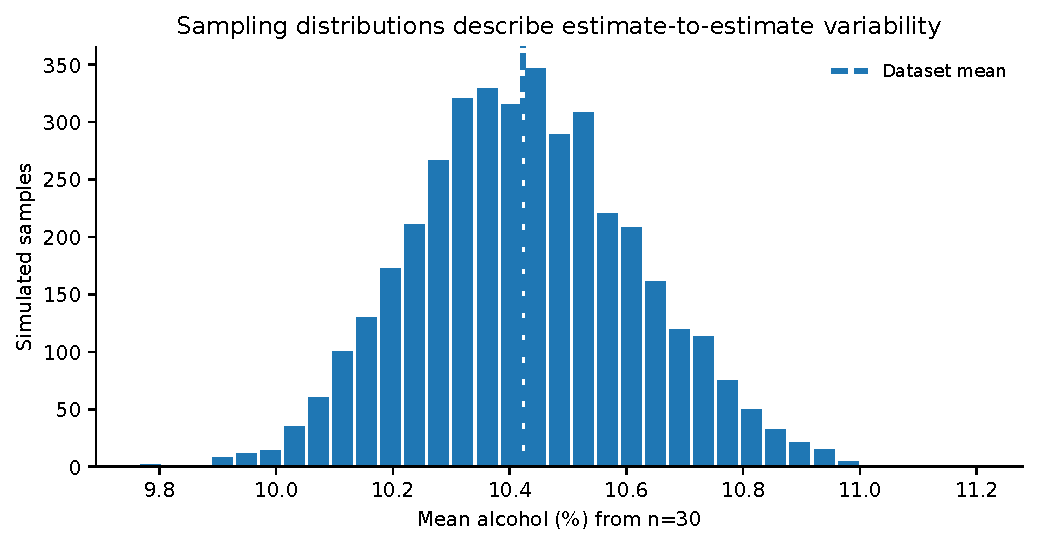
\includegraphics[width=0.84\linewidth]{figures/inference_sampling_distribution.pdf}
\end{utpfig}

\section{Standard error describes estimate-to-estimate variability}
The \term{standard error} is the standard deviation of a statistic's sampling distribution. For a sample mean under familiar assumptions,
\[
SE(\bar{x}) \approx \frac{s}{\sqrt{n}}.
\]
The square-root relationship is important: quadrupling sample size roughly halves the standard error, all else equal. This gain in precision does not remove bias from poor sampling or measurement.


\section{Bias and variability are different problems}
A large convenience sample can estimate the wrong population very precisely. More observations reduce random variability, but they do not automatically repair selection bias, measurement bias, or confounding.

\section{Bootstrap confidence intervals}
The bootstrap approximates sampling variability by repeatedly resampling the observed data with replacement.

\begin{utpsteps}
  \item Compute the statistic of interest on the observed sample.
  \item Resample the rows with replacement to create a bootstrap sample of the same size.
  \item Recompute the statistic and store it.
  \item Repeat many times; use the bootstrap distribution to form an interval.
\end{utpsteps}

\begin{lstlisting}[style=utpr]
set.seed(42)
boot_means <- replicate(
  2000,
  mean(sample(wine$alcohol, replace = TRUE))
)
quantile(boot_means, c(0.025, 0.975))
\end{lstlisting}


\begin{utpfig}[Bootstrap distribution]{Bootstrap resamples mimic repeated sampling from an empirical approximation to the population. The central 95\% of the resampled means gives a simple percentile interval.}{fig:inference-bootstrap}
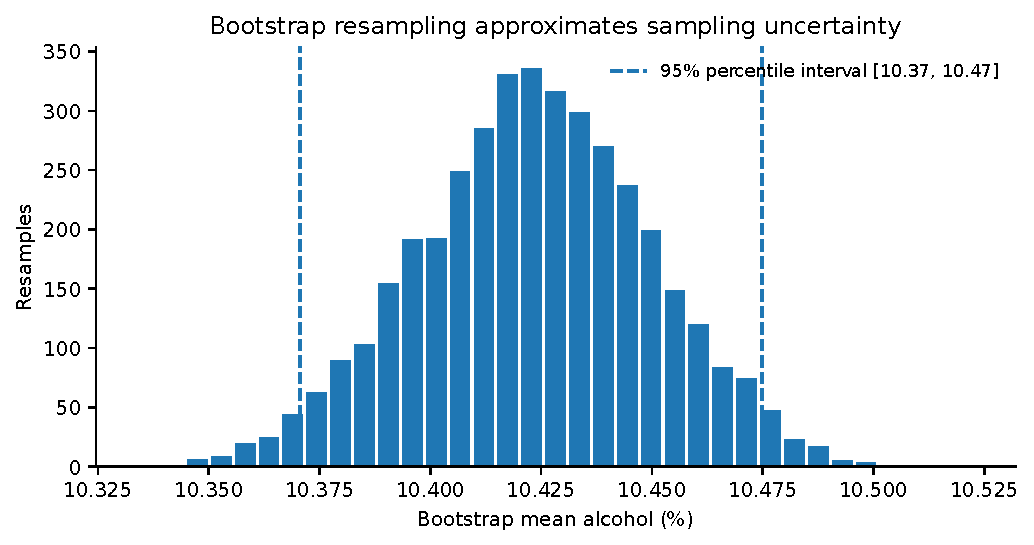
\includegraphics[width=0.84\linewidth]{figures/inference_bootstrap.pdf}
\end{utpfig}

\section{Confidence intervals quantify a range of compatible values}
A 95\% confidence interval is produced by a procedure designed to cover the target parameter about 95\% of the time under repeated sampling and the method's assumptions. Once a particular interval has been calculated, the parameter is fixed; the frequentist interpretation concerns the long-run procedure rather than a 95\% probability assigned to that fixed parameter.

\begin{utpfig}[Repeated-sampling interpretation of confidence intervals]{Most intervals in this simulation cross the dashed population mean; occasional intervals miss it. This long-run behaviour is what confidence level describes.}{fig:inference-ci-coverage}
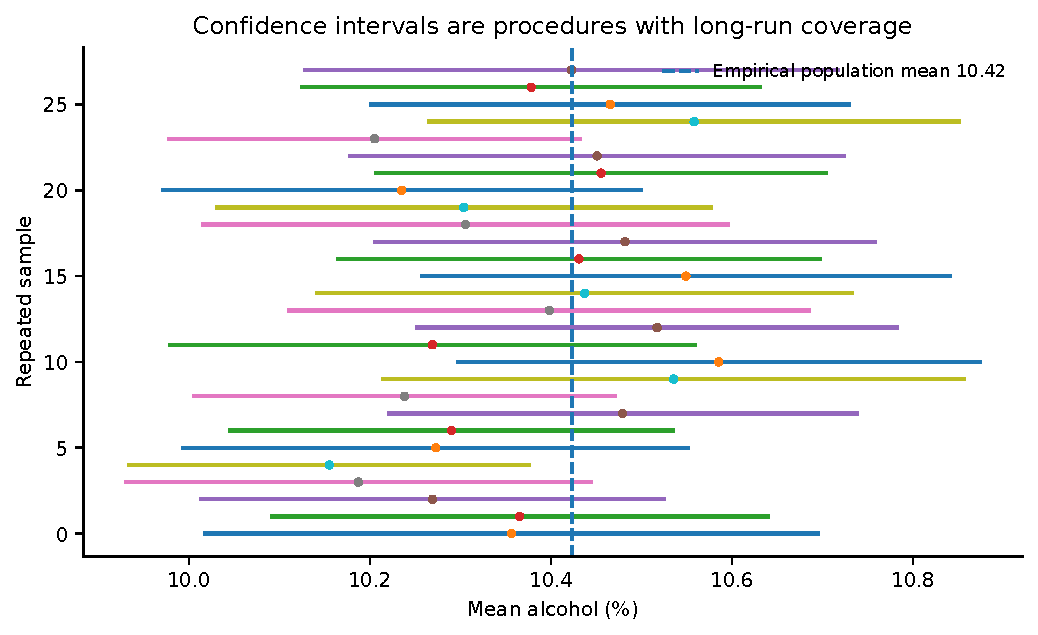
\includegraphics[width=0.82\linewidth]{figures/inference_ci_repeated.pdf}
\end{utpfig}

\section{Hypothesis tests compare data with a null model}
A p-value is the probability, under a specified null hypothesis and test assumptions, of obtaining a result at least as incompatible with the null as the observed result. It is not the probability that the null hypothesis is true.

\begin{pitfall}
``Statistically significant'' does not mean ``important'', ``large'', or ``causal''. With enough data, a tiny difference can have a small p-value. Always report the magnitude and practical meaning of the effect.
\end{pitfall}


\section{A hypothesis test has several moving parts}
A disciplined test states the null and alternative hypotheses, chooses a statistic, checks assumptions, computes the statistic's null reference distribution or approximation, and then interprets the p-value in context. The p-value is sensitive to both effect size and sample size, which is why it should not be used as a stand-alone measure of scientific importance.

For a two-group comparison, also inspect group distributions and report an effect such as a difference in means or medians in original units. If a standardised effect size is useful for comparison across scales, explain what its units mean.


\section{Effect size and uncertainty belong together}
For a difference in means, report the observed difference in original units and an interval or test that describes uncertainty. Readers can then judge both size and precision.

\begin{workedexample}
Suppose two wine cultivars differ in mean alcohol measurement. The t-test addresses compatibility with a zero-difference model; the actual difference in alcohol units tells the reader whether the magnitude is meaningful in context.
\end{workedexample}


\section{Multiple testing increases false discoveries}
If an analyst tests many unrelated hypotheses and reports only those with small p-values, some apparently ``significant'' results can arise by chance. Pre-specifying primary questions, correcting for multiplicity when appropriate, and validating exploratory findings on new data reduce this risk.

\begin{pitfall}
A confidence interval or p-value quantifies uncertainty conditional on assumptions. It does not automatically account for selection bias, measurement error, poor operational definitions, unrecorded exclusions, or the fact that the hypothesis was chosen after inspecting the same data.
\end{pitfall}


\section{Study design limits causal claims}
Randomised experiments can isolate treatment effects when implemented well. Observational data can describe associations and support prediction, but causal interpretation requires stronger assumptions and methods than correlation or regression alone.

\begin{keyidea}
Inference is not a machine for turning samples into certainty. It is a framework for expressing what the data say while keeping sampling and design uncertainty visible.
\end{keyidea}

\begin{quickcheck}
\begin{enumerate}
  \item What is the difference between sampling variability and selection bias?
  \item What does resampling with replacement accomplish in the bootstrap?
  \item What does a p-value \emph{not} tell you?
  \item Why should effect size accompany statistical significance?
\end{enumerate}
\end{quickcheck}

\section{Worked inference: student performance and observational uncertainty}

In the Student Performance dataset, mean final grade \texttt{G3} is about 12.28 among students who report an intention to pursue higher education and about 8.80 among those who do not---an observed difference of roughly 3.48 grade points.

\begin{utpfig}[Bootstrap distribution for a mean difference]{Resampling students within the observed groups approximates the sampling variability of the group mean difference under the empirical distribution. The interval describes uncertainty in the estimate, not uncertainty about unmeasured confounding.}{fig:inference-student-bootstrap}
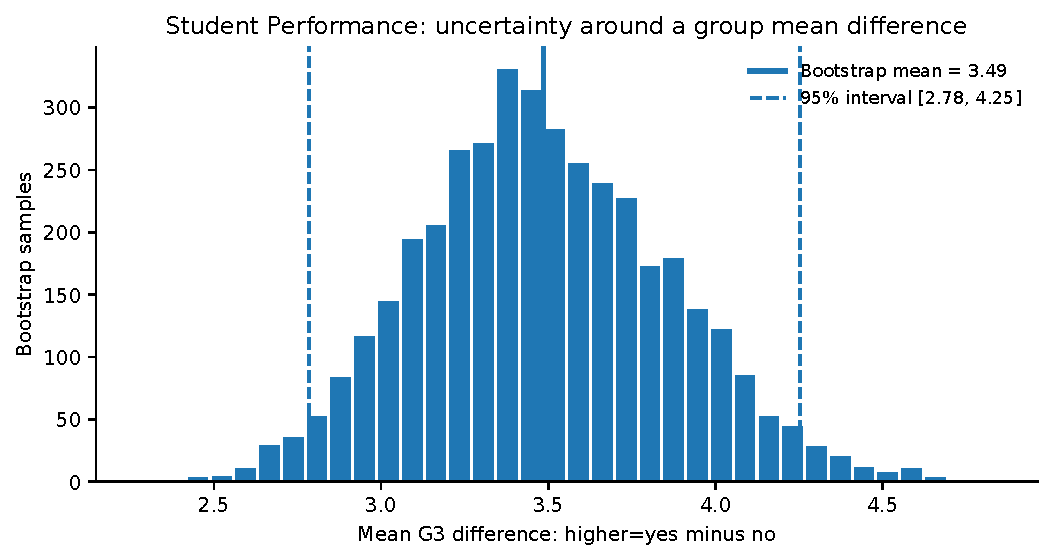
\includegraphics[width=0.86\linewidth]{figures/inference_student_bootstrap.pdf}
\end{utpfig}

This example separates three questions that students often merge. \textbf{Estimation} asks how large the observed difference is. \textbf{Sampling uncertainty} asks how much that estimate might vary under repeated sampling. \textbf{Causal interpretation} asks whether changing higher-education intention would change grades. Bootstrap intervals help with the second question; they do not solve the third.

Potential confounders include prior grades, study time, parental education, school support, failures, and socioeconomic context. Formal uncertainty can be numerically precise while the causal claim remains weak.


\section{Bootstrap and permutation answer different questions}

The Student Performance example is useful because two resampling procedures can be placed side by side. The bootstrap resamples within the observed groups and asks how much the estimated mean difference would vary if similar samples were collected again. A permutation procedure instead breaks the link between group label and outcome and asks how unusual the observed contrast is under an exchangeability-based no-association reference model.

\begin{utpfig}[Permutation inference creates a null reference distribution]{The shuffled-label distribution is centred near zero because the group labels have been deliberately detached from final grades. The observed difference is then compared with this reference distribution.}{fig:inference-student-permutation}
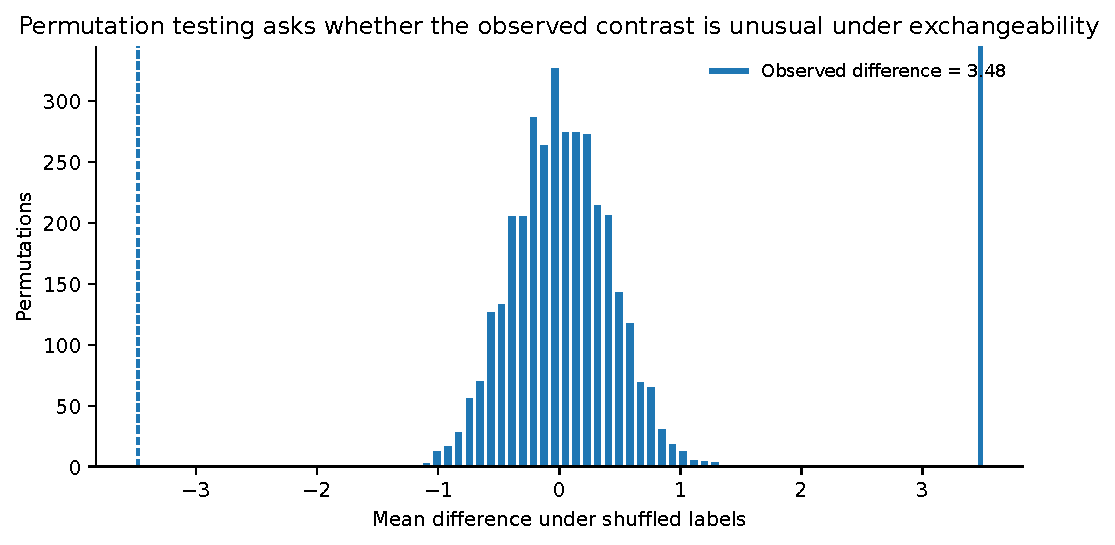
\includegraphics[width=0.82\linewidth]{figures/inference_student_permutation.pdf}
\end{utpfig}

The procedures are related but not interchangeable. The bootstrap is primarily an estimation tool here; the permutation distribution is a testing tool. Both inherit assumptions from the sampling process, and neither makes the observational comparison causal. This is why a complete inference statement should report the \textbf{effect size}, the \textbf{uncertainty or reference distribution}, and the \textbf{design limitation} in separate sentences.
